\documentclass[uplatex]{jsarticle}
\usepackage[dvipdfmx]{graphicx}
\usepackage{ascmac}
\usepackage{listings}
\usepackage{amsmath}
\usepackage{bm}
\usepackage{cases}

\DeclareMathOperator*{\minimize}{minimize}


\title{人工知能 課題番号1「人工知能の実現可能性について考察せよ」}
\author{工学部電子情報工学科 03-175001 浅井明里}

\makeatletter
\def\maketitle{%
  \null
  \thispagestyle{empty}%
  \vfill
  \begin{center}\leavevmode
    \normalfont
    {\LARGE \@title\par}%
    \vskip 1cm
    {\Large \@author\par}%
    \vskip 1cm
    {\Large \@date\par}%
  \end{center}%
  \vfill
  \null
  \@thanks%\vfil\null
  \cleardoublepage
  }
\makeatother


\title{人工知能 課題番号08「幾何図形類推問題」}
\author{工学部電子情報工学科 03-175001 浅井明里}
\date{\today}

\begin{document}
\maketitle

\section{EvansのプログラムANALOGYがどのように幾何図形類推
問題を解くことができたか}
類推(Analogy)とは、ある物事と別の物事の間の何らかの類似に基づいて一方がある性質を持つ場合に
他方もそれと同じ性質を持つであろうと推理することであり、EvansのANALOGYプログラムは
この幾何の類推を行う古典的なプログラムである。
ANALOGYでは以下のようなステップで幾何類推問題を解く。
\begin{enumerate}
  \item それぞれの問題の図を複数の"Object(sub figure)"に分解し、その関係を記号表現に直す。
  \item 記号的な表現のマッチングを行う。
  \item ある幾何図形からある幾何図形に変換するルールを生成する。
\end{enumerate}

この項では、このALNALOGYプログラムがどのようにして幾何類推
問題を解いていたのかを以下の図1の例を元に紹介していきたい。
\begin{figure}
  \begin{center}
    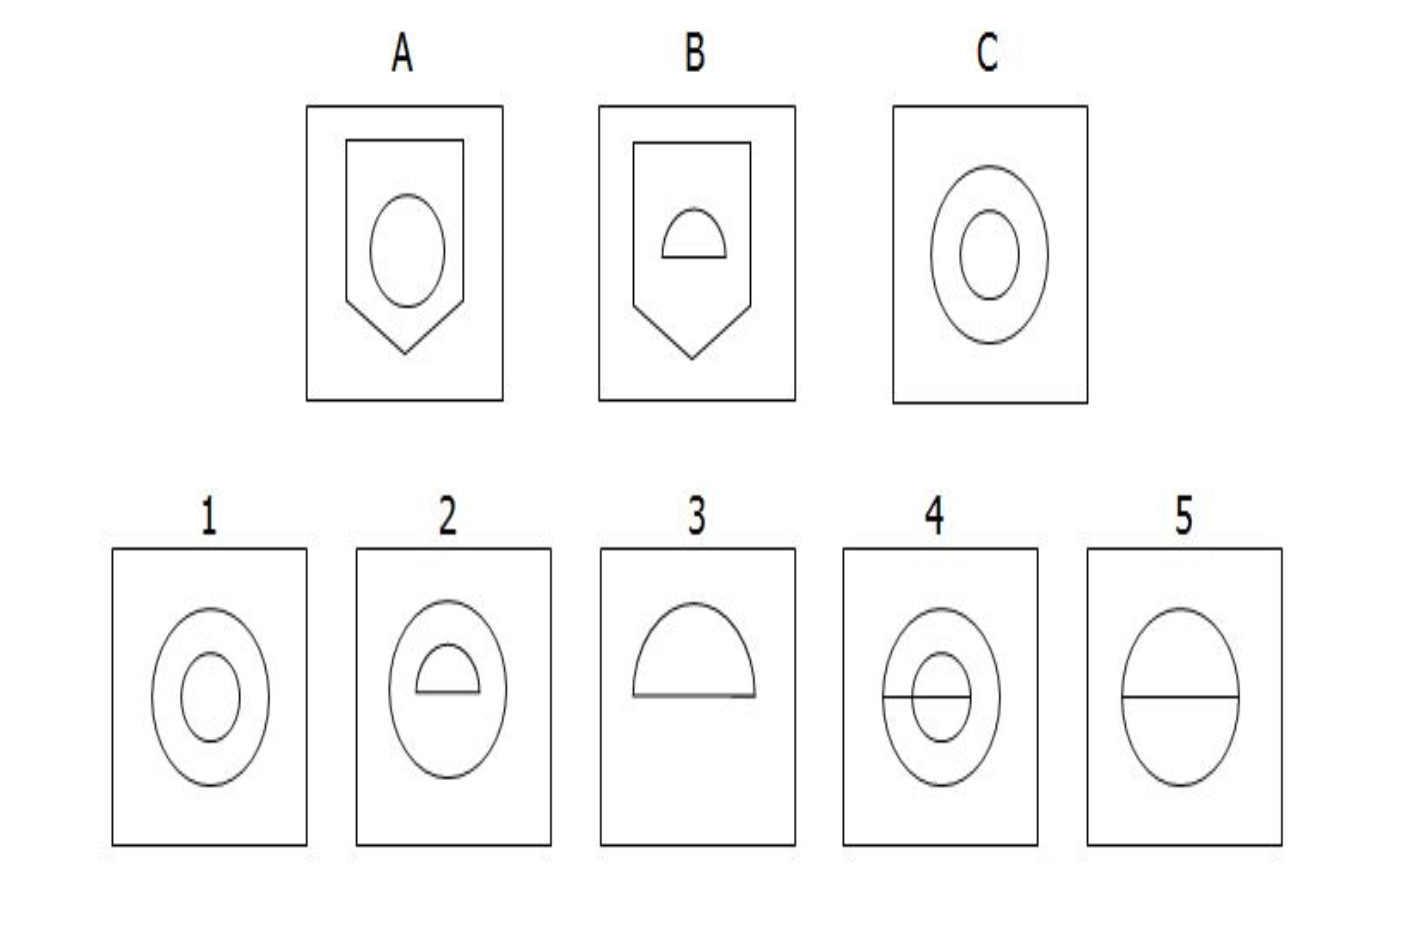
\includegraphics[width=10cm]{img/problem.png}
    \caption{幾何類推問題の例}
  \end{center}
\end{figure}

\subsection{図A, B, Cの類似点と相違点を記述するプログラムでは、各図をどのように記述すれば良いか}
まず、図A、B、Cをそれぞれ記号表現で記述する。記述の仕方についてはANALOGYを提案した論文及び参考書
より、図に含まれるオブジェクトを列挙するCONSISTS-OF, またそれぞれのオブジェクトの関係性を記述する
RELATIONSで表現し、またRELATIONSについてはINSIDE, ABOVEの二種類で表現し、
(INSIDE SubFig1 SubFig2)ならばSubFig1がSubFig2に含まれていることを、
(ABOVE SubFig1 SubFig2)ならばSubFig1はSubFig2の上方にあることを表すとする。
またそれぞれのオブジェクトに以下の図2のように識別のための名前をつけることとする。

\begin{figure}
  \begin{center}
    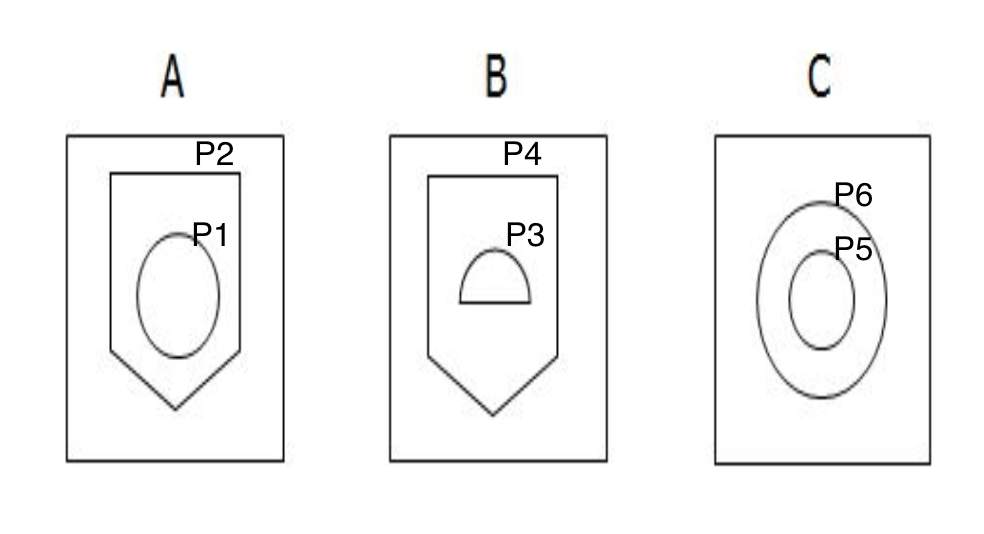
\includegraphics[width=10cm]{img/abc_comparison.png}
    \caption{幾何類推問題の例}
  \end{center}
\end{figure}

\begin{lstlisting}[basicstyle=\ttfamily\footnotesize, frame=single]
  (FIG A
          (CONSISTS-OF P1 P2)
          (RELATIONS (INSIDE P1 P2)))
  (FIG B
          (CONSISTS-OF P3 P4)
          (RELATIONS (INSIDE P3 P4)))
  (FIG C
          (CONSISTS-OF P5 P6)
          (RELATIONS (INSIDE P5 P6)))
\end{lstlisting}

次に、A、B間の類似性、AとCの間の類似性を記号から推定する。あるFigure1からFigure2に類似性は(SIM-Figure1-Figure2)と表し、
そのうち特にFigure1に含まれるSubFigure1-1からFigure2に含まれるSubFigure2-1に変換が可能であるとき、
変換情報は(TRANS a b c d)で表現される。
このときa,b,c,dはそれぞれ以下の変換情報を示している。
\begin{itemize}
  \item a, d : 対象変換の種類。
  \begin{itemize}
    \item K : 鏡像
    \item V : 垂直
    \item H : 水平
  \end{itemize}
  \item b : 相似変換の拡大率
  \item c : 回転変換の角度
\end{itemize}

\begin{lstlisting}[basicstyle=\ttfamily\footnotesize, frame=single]
  (SIM-A_B (SIM P2 P4 : (TRANS K 1.0 0 K)))
  (SIM-A_C (SIM P1 P5 : (TRANS K 1.0 0 K)))
\end{lstlisting}
以上よr、AとBにおいてP2とP4が、AとCにおいてP1とP5が類似であることが導かれる。
\subsection{図Aを図Bに変える規則の記号的な記述を与え、この規則を上で与えた記述からどのように機械的につくることができるかを説明せよ。}
前項で求めた類似性の記号表現より、図Aを図Bに変える規則の記号的な表現を求める。変形の手順については以下のように記述する。
\begin{itemize}
  \item $\bf{REMOVE\ SubFigure1\ WITH\ (ConditionsA)}$  \\ ConditionAに合致するSubFigure1を取り除く。
  \item $\bf{MATCH\ SubFigure2\ FROM\ (ConditionsB)}\ TO\ (ConditionsC)\ WITH\ (TRANS\ a\ b\ c\ d)$  \\ SubFigure2を  変換情報TRANSを維持したまま、条件ConditionBから条件ConditionC
  を満たすように変更しする。
  \item $\bf{ADD\ NewFigure1\ WITH\ (ConditionsA)}$  \\  NewFigure1を条件ConditionsAを充しながら追加する。
\end{itemize}
この規則を与えた上で、前述の図AとBの類似関係から機械的に導くと、変更規則の記号的な記述は次のようになる。これは以下のような手順で機械的に求めることができる。

オブジェクトP2とP4は類似しており、追加も削除も必要なくまた図形的にも全く同じ像であるため変換規則の適用も必要ない。
次にP1とP3であるが、この二つの図形に類似性はなく(P1を半分に分割したものがP2と捉えることもできるが、この問題ではこの二つの図形を類似性のない独立したものであると捉えることとする)、図Aから図Bの変換にはP1を除去し、
P3を追加する必要があることがわかる。P1を特定する条件をWITH以下に記述し、また(SIM OBJ3 ...)は図Aと図Bの
図形の種類を比較するための方法を示している。
最後に新たな図形P3を追加する部分では、追加する際の条件(この場合は既存するもう一方の図形の内部に配置する)と共に図形を追加する旨を記述する。
最終的に変換規則は以下のように表現できる。
\begin{lstlisting}[basicstyle=\ttfamily\footnotesize, frame=single]
((REMOVE x1 WITH ((INSIDE x1 x2)
                (SIM OB3 x1 (TRANS K 1.0 0 K)))
(ADD x2 WITH ((INSIDE x2 x3))))
\end{lstlisting}
以上の手順により、図形Aから図形Bへの変換規則が機械的に示された。

\subsection{自分の作った規則を図Cに対して自分の作った記述に適用せよ。その結果どのような記述が得られ、それはどのような図であるかを説明せよ。この図と図Cとの間の類似点を記述せよ。}
以上の変換規則を、図Cに適用した場合以下のように記述でき、すなわち図Cに含まれる二つの図形のうち、一方のより大きな図形に含まれるもう一方の図形を除去し、
新たな図形を残っている図形の内部に追加すればいいということがわかる。
\begin{lstlisting}[basicstyle=\ttfamily\footnotesize, frame=single]
((REMOVE P5 WITH ((INSIDE P5 P6)
                (SIM OB3 x1 (TRANS K 1.0 0 K)))
(ADD Px WITH ((INSIDE Px x6))))
\end{lstlisting}
新たな図形X及びCとXの類似性は次のような記号的表現記述により表すことができ、結果としてANALOGYプログラムに図1のような問題を与えたとき、
得られる答えは図1の「2」となることがわかる。

\begin{lstlisting}[basicstyle=\ttfamily\footnotesize, frame=single]
  (FIG X
          (CONSISTS-OF P7 P8)
          (RELATIONS (INSIDE P7 P8)))
  (SIM-C_X (SIM P6 P8 : (TRANS K 1.0 0 K)))
\end{lstlisting}

\subsection{図Cの記述方法を変えて、同じ規則をその記述に適用すると、前とは違った結果になるようにせよ。}
次に、図Cの記述方式を以下のように変換する。
\begin{lstlisting}[basicstyle=\ttfamily\footnotesize, frame=single]
  (FIG C
          (CONSISTS-OF P6 P5)
          (RELATIONS (INSIDE P5 P6)))
\end{lstlisting}
この図Cの記述に基づいて、図Aと図Cの類似性を記号的に表現する場合、以下の通りになる。
\begin{lstlisting}[basicstyle=\ttfamily\footnotesize, frame=single]
  (SIM-A_C (SIM P1 P6 : (TRANS K 0.8 0 K)))
\end{lstlisting}
すなわち、図Cの表現方法を変化させたことで図Aとのオブジェクトの対応関係が変化し、その結果図Aと図Cの類似性の記述に変化
が生じた。
図AのP1に対応する、すなわち返還後除去されることとなるオブジェクトはP6となり、P5は除去されることなく残存し、
新たなオブジェクトはこのP5の内部に存在することになる。
\begin{lstlisting}[basicstyle=\ttfamily\footnotesize, frame=single]
  (FIG X
          (CONSISTS-OF P7 P8)
          (RELATIONS (INSIDE P7 P8)))
  (SIM-C_X (SIM P5 P8 : (TRANS K 1.0 0 K)))
\end{lstlisting}
結果として返還後に得られる図は前項の回答と一回り小さい図形となることがわかる。

\subsection{EvansのプログラムANALOGYでは解くことができないであろう幾何図形類推問題の例を示し、なぜ解けないのかを説明せよ。}
Evansのプログラムでは解くことのできない問題の例をいくつかあげたいと思う。

Evansのプログラムにおいて、図に含まれるそれぞれのオブジェクトは二つの図を比較するとき
図に含まれるオブジェクト同士が互いに一対一で対応する必要がある。しかし、例えば「図Aにおいて二つのオブジェクトが与えられており、それらを
結合すると図Bとなる」というような変換規則であった場合、ANALOGYによる幾何類推では、図A及び図Bの間のそれぞれのオブジェクト間に
一対一関係を構築することができないため、正しく類推をすることができない。以下で例を示す。

\begin{figure}[htbp]
\begin{minipage}{0.4\hsize}
 \begin{center}
  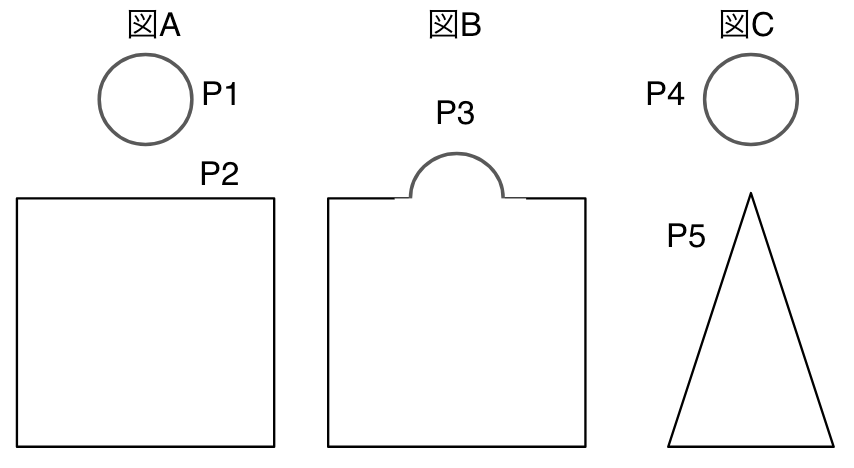
\includegraphics[width=60mm]{img/example1.png}
 \end{center}
 \caption{正しく類推ができない問題の例}
 \label{fig:one}
\end{minipage}
\begin{minipage}{0.6\hsize}
 \begin{center}
  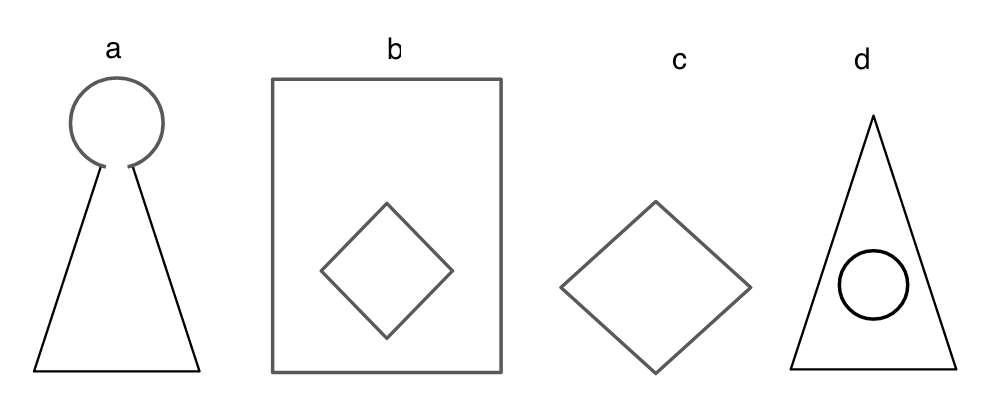
\includegraphics[width=80mm]{img/sol.png}
 \end{center}
 \caption{ANALOGYで正しく類推ができない問題の選択肢}
 \label{fig:two}
\end{minipage}
\end{figure}

図3のような例が与えられれば、人間であれば、「図Aには丸と四角形が存在しており、
図Bに変換するためにはこの二つの図形を結合させれば良い。よって、図Cに同様の変換規則を
適用すれば、三角形と丸という二つのオブジェクトが結合し、図4の(a)となる」と類推できるであろう。
ANALOGYでこの問題を解こうとして場合それぞれの図及びそれらの類似性は以下のように表現される。
\begin{lstlisting}[basicstyle=\ttfamily\footnotesize, frame=single]
(FIG A (CONSISTS-OF P1 P2)
       (RELATIONS (ABOVE P1 P2)))
(FIG B (CONSISTS-OF P3))
(FIG C (CONSISTS-OF P4 P5)
      (RELATIONS (ABOVE P4 P5)))

(SIM-A_B ())
(SIM-A_C
          (SIM P1 P4 : (TRANS K 1.0 0 K)))
\end{lstlisting}

ANALOGYでは図に含まれるオブジェクトを分離する際、重なっている図形については単一閉曲線の図形になるように分離すれば良いとしたが、
この方式で図A, B, Cを見るとき、A, Cについてはそれぞれ丸と正方形、丸と三角形という二つのオブジェクトに分離が可能だが、
Bについては正方形に丸が結合された図形であっても、これはP3という単一のオブジェクトとして考えられることとなる。
その結果、図形AとBの間の類似性を見つけようにもAの二つのオブジェクトと類似する図形は存在しないため見つけることができない。
故に、AからBへの変換規則は次の通りとなる。

\begin{lstlisting}[basicstyle=\ttfamily\footnotesize, frame=single]
(REMOVE x1 WITH ((ABOVE x1 x2)
                (SIM OB3 x1 (TRANS K 1.0 0 K)))
(REMOVE x2 WITH ((ABOVE x3 x2)
                (SIM OB3 x1 (TRANS K 1.0 0 K)))
(ADD x3 ())
\end{lstlisting}

すなわち、図に存在する二つのオブジェクトを除去し、新しいオブジェクトを追加するというのが変換規則となってしまい、
この場合類推の結果提示される回答は(c)となるがこれは誤った類推結果である。
またこの問題は結局のところANALOGYプログラムにとって図AとBが全く異なる図形として解釈された場合、
ANALOGYは正しい類推結果を出すことができないことも暗示している。

また、オブジェクトが複数のアトリビュート(形、位置関係、パターン、色等)を持つ問題もANALOGYプログラムでは
正しい類推結果を求めることが難しいのではないかと推測する。例として図5に示された問題について考えたい。
図形を記号的表現に落とし込むに当たって、新たにPATTERNというアトリビュートを導入したい。PATTERNにはSTRIPE, DOT, PLAIN
という3種類の柄のいずれかが全ての図形に対して与えられる。

\begin{figure}
  \begin{center}
    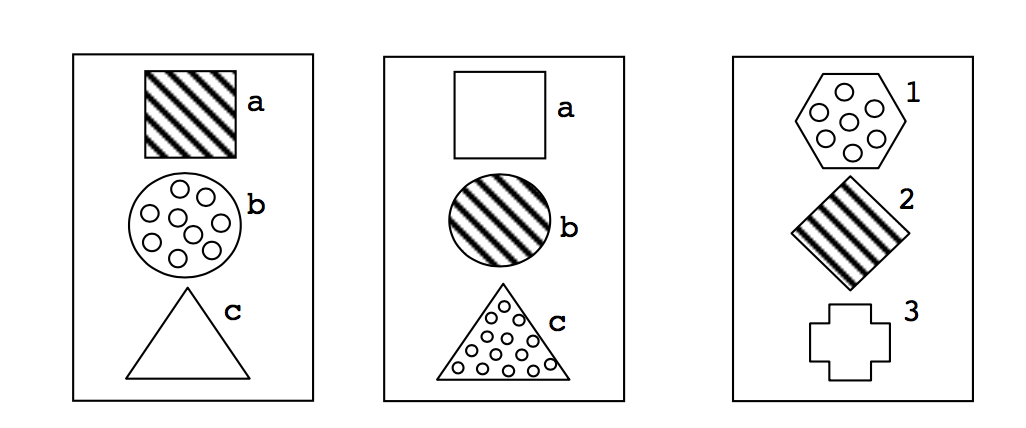
\includegraphics[width=13cm]{img/difficult_example2.png}
    \caption{幾何類推問題の例}
  \end{center}
\end{figure}

\begin{lstlisting}[basicstyle=\ttfamily\footnotesize, frame=single]
(FIG A (CONSISTS-OF P1 P2 P3)
       (RELATIONS (ABOVE P1 P2)(ABOVE P2 P3))
       (PATTERN (STRIPE P1)(DOT P2)(PLAIN P3))

(FIG B (CONSISTS-OF P4 P5 P6)
       (RELATIONS (ABOVE P4 P5)(ABOVE P5 P6))
       (PATTERN (PLAIN P1)(STRIPE P2)(DOT P3))

(FIG C (CONSISTS-OF P7 P8 P9)
       (RELATIONS (ABOVE P7 P8)(ABOVE P8 P9))
       (PATTERN (DOT P1)(STRIPE P2)(PLAIN P3))
\end{lstlisting}

ここで問題となるのは、オブジェクト同士の一対一対応関係を求めるにあたりRELATIONSとPATTERNという
二つのアトリビュートのうち、どちらが優先されるべきかが明示されていないためRELATIONSを優先させた
類推結果とPATTERNを優先させた類推結果の複数種類の結果が導き出されることとなる。

他にANALOGYが解くことのできない類推問題として、「数え上げ」「背景の反転」等、事前に機能として想定されていれば
類推可能だが、そうでなければ解くことのできない問題が想定される。図6で示された例では
「図Aにあるオブジェクトの数が図Bで数字で示される」という変換規則が成立し、これを一番
右の図に適応すると、この図は二つのオブジェクトを持つため変換後は数字の「2」が
中央に配置された図になるべきだと予測できる。しかし前述の記号的表現及びANALOGYの
機能では、こういったオブジェクトの数を数え、それによって追加するオブジェクトを
決定する機能はなくこの問題を解くことができない。

\begin{figure}
  \begin{center}
    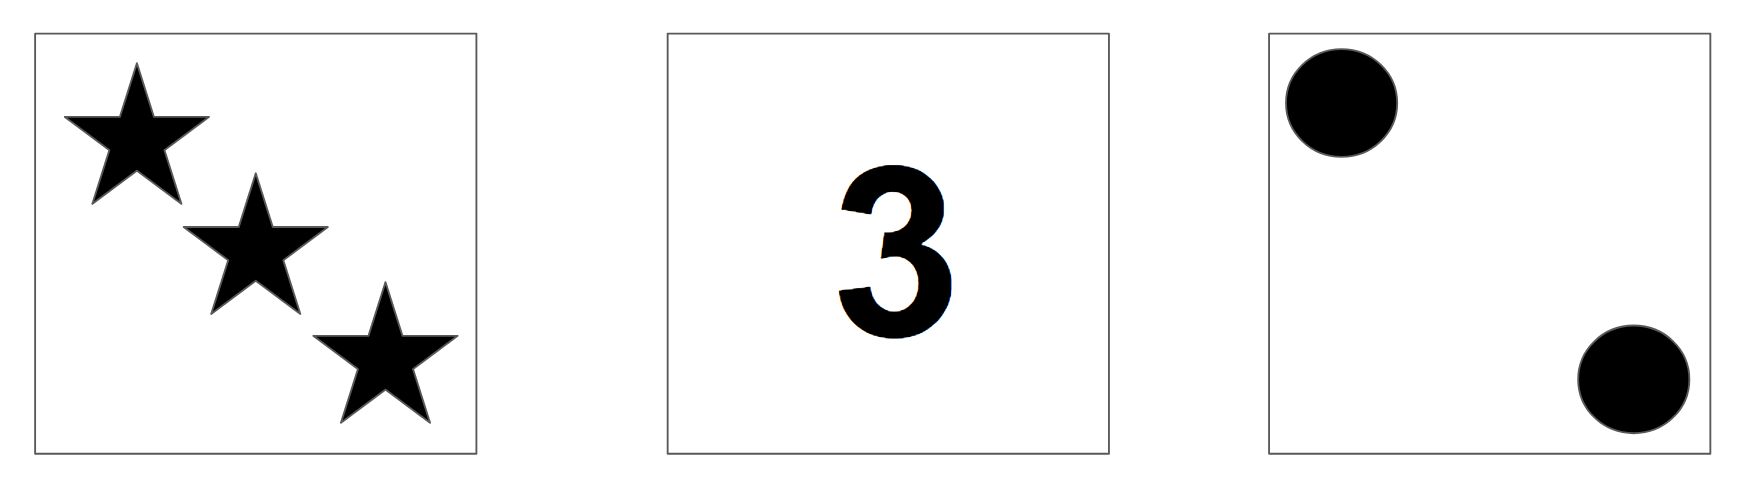
\includegraphics[width=13cm]{img/numbering.png}
    \caption{幾何類推問題の例}
  \end{center}
\end{figure}

また図7の問題に存在する変換規則は「図のオブジェクトの色と背景色を反転させる」というものだと推測できるが
上述の記号的表現ではこの「色の反転」に相当する表現は定義されておらず、
既存の色やパターンのみで判断することも前述の複数マッチングの観点より困難であり、
やはり正しい類推を行うことのできない可能性がある。

\begin{figure}
  \begin{center}
    
\includegraphics[width=13cm]{img/inverse.png}
    \caption{幾何類推問題の例}
  \end{center}
\end{figure}


\subsection{EvansのプログラムANALOGYとIQテストに用いられるような幾何図形類推問題に関する以下の命題について、上で示した例などを利用して論ぜよ。}
\subsubsection{幾何学的図形類推問題を解く知的行為の基本的な要素は、純粋に機械的なものであることを示した。}
幾何学的図形類推問題を解く知的行為の基本的な要素は純粋に機械的なものではないと私は考える。
類推を行う際、まず最初に図形及びそれらの類似性を記号的表現で示す必要がある。与えられた図形画像を認識し、
ある程度機械的にこの作業を行うことは現在の技術では可能かもしれないが、仮にそうであった場合にもいくつかの問題点が存在していると考える。

第一の問題はある図形を複数のオブジェクトに分解し、図形同士の関係性も合わせて記号的表現
に落とし込む段階にあると考える。図を複数のオブジェクトに分解する際に、「単一閉曲線」で図形を区切ることが可能かどうか与えられた問題に依存しており、
例えば前述のようなオブジェクト同士が結合してしまった図の場合、人間ならば隠れた線を推測し無意識にその図形が丸と四角の結合したものだと認識できるが
類推プログラムの場合明示的にこのルールも追加しなくては正しくオブジェクトに分解することができなくなる。ただこのとき、どの場合では単一閉曲線を二つのオブジェクトが
結合したものと認識するのか、例えば菱形は三角形が二つ結合したものと考えるべきなのか等多くの条件の設定が必要となり、
結果的に人手である程度オブジェクトの分解についてのルールを与える必要があり機械的に図形を記号的表現に正しく変換可能だとは考えらない。

第二の問題は複数のアトリビュートを持つ図形の類似性の記述におけるアトリビュートの優先順位に関する問題である。
図5の問題のような、図に含まれるオブジェクトが複数のアトリビュートを持つ際にこのアトリビュートの優先順位をどう付けて
図同士の対応関係を求めるか、図形の変換を行うかにより答えが変わってしまう。Bohan(2000)らはこの問題に対し、
オブジェクトのペアに対して適用されるlocalアトリビュート変換と全てのオブジェクトに対して
適用されるglobalアトリビュート変換という異なるアトリビュート変換を用い、この問題の解決を試みた。
ただ解決法についても、アトリビュートの優先順位付についても人の手により明確に「基準」を与える必要があり、完全に機械的に行うことができない。

以上より、幾何学的図形類推問題を解く知的行為の基本的な要素は純粋に機械的なものではないと私は考える。

\subsubsection{幾何学的図形類推問題を解くのに必要な知的な能力は、もとになる記号的記述体系をどのように選ぶかというところにのみ存在する}
幾何学的図形類推問題を解くのに必要な知的な能力は、もとになる記号的記述体系をどのように選ぶかというところにのみ存在するという命題は偽りであると
私は考える。仮に元となる記号的記述体系を決定できたとしても、幾何類推のためにはそれ以外にも機械的に
解くことのできない段階が存在するためである。記号的記述体系以外に必要だと私が考える知的能力は以下の二つがある。

まず、あらかじめ定められた記号的記述体系で表現し得ないような問題に直面した時、
現在自分の持つ機能、記号的表現だけでは十分にその問題に対し正しい幾何類推を行うことができないと
判断できる能力である。数え上げ問題、反転問題等は問題中の図自体を記号的表現に落とし込むことは既に定義された
記号的表現で十分に可能である。しかし一方で、数え上げ問題を「全てのオブジェクトを除去し、必ず1個のオブジェクトを中央に配置する」
と解釈してしまったり、反転を「グローバルなトリビュートの変換」と解釈してしまった場合、おそらく問題で想定された解を導くことは難しい。
ここで必要なのは問題に直面する度に、まず自身の持つ記号的表現を適用してみるのではなく、そもそもこの問題は自身の今現在持つ
アプローチで正しく回答ができるのかを判断する知的能力が必要である。

次に与えられた問題に既存の機能、記号的表現では十分に対応できないと判断した場合、
自ら新たに必要な記述体系を生み出し類推をすることである能力である。
そこで既に獲得している記号的記述体系等を参考にしつつ新たな記述体系、機能を生み出していく必要があり、
この場面においても知性は必要である。

この点に対して、全ての問題を解くために必要な機能、記号的表現をあらかじめ全てプログラムしておけばいいのではないかという
反駁も想定できるが、
どのような幾何類推問題が聞かれうるか全てあらかじめ想定仕切ることは不可能であり、また新たに生み出される
問題に対して十分に対応できるものでなければ幾何類推問題を適切に解くことのできるプログラムだということはできない点で
全ての問題を想定するという前提が実現性のないものであるためこの反駁は不十分である。

以上より、幾何学的図形類推問題を解くのに必要な知的な能力は、
もとになる記号的記述体系をどのように選ぶかというところにのみ存在するという命題は偽りであると私は考える。


\begin{thebibliography}{9}
  \bibitem{evans} Thomas G. Evans,
    "A HEURISTIC PROGRAM TO SOLVE GEOMETRIC-ANALOGY PROBLEMS", Air Force Cambridge Research, Laboratories (OAR) Bedford, Massachusetts, 1968.
  \bibitem{iba} 伊庭斉志,
    『人工知能と人工生命の基礎』, オーム社 , 2013.
% http://www.orsj.or.jp/~archive/pdf/bul/Vol.32_09_606.pdf
  \bibitem{LUDI} A. Bohan, D. O'Donoghue, "LUDI: A Model for Geometric Analogies using Attribute Matching",
  Dept. Computer Science, NUI Maynooth, Co. Kildare, Ireland, 2000.
  % http://www.cs.nuim.ie/~dod/pubs/00-aics.pdf
\end{thebibliography}


\end{document}
